\section{Konsolidation}
%\begin{minipage}{0.5\linewidth}
%	\renewcommand{\arraystretch}{2}
%\begin{alignat*}{2}
%	\text{Dehnung} 		& \qquad	&  \epsilon &= \frac{\Delta h}{h_0}  \\
%	\text{Porenziffer}  &&  e_0 		&= \frac{\gamma_s}{\gamma_d} -1  \\
%						&&  e 			&=e_0-\epsilon \cdot \left(1+ e_0\right) \\
%	&\rightarrow&  \frac{\Delta h}{h} 	&= \frac{e_0 - e}{1+e_0} 	\\		
%	&\rightarrow& \Delta h 				&= \frac{\Delta \sigma \cdot h_0}{M_E} \\
%	M_E-Modul	&&  M_E					&=\frac{\Delta \sigma}{\Delta \epsilon}=\frac{1+e_0}{C_c \cdot 0.434}\cdot\sigma_m \\	
%	&\rightarrow &  \gamma_d			&=\frac{\gamma}{1+w} \\
%				&& n&=\frac{\gamma-\gamma_d}{S_r\cdot\gamma_w} \\
%				&& e_0&=\frac{n}{1-n} \\
%				&& \gamma&=\frac{G}{V}\cdot g \\
%				&& \gamma_s&=16-17 \; kN/m^3 \\
%	\rightarrow Oedometer && \sigma&=M_E \cdot \epsilon \\
%				& \rightarrow& M_E&\neq E, \hspace{0.25cm}\text{da} \hspace{.25cm} \epsilon_2=\epsilon_3=0 \\
%				&& \sigma_m&=\frac{2\cdot\sigma_0+\Delta \sigma}{2} \\
%	Konsolidationskoeffizient [cm^2/s]&&  C_v&=\frac{M_E\cdot k}{\gamma_w}=\frac{T_v\cdot d^2}{t} \\
%	\text{Durchlässigkeitswert} && k&=\frac{C_v\cdot\gamma_w}{M_E} \\
%	Zeitfaktor	&& T_V&=\frac{t\cdot C_V}{d^2}=\frac{t\cdot M_E\cdot k}{\gamma_w\cdot d^2} \\
%\end{alignat*}
%\renewcommand{\arraystretch}{\arraystretchOriginal}
%\end{minipage}
%
%\begin{minipage}{0.5\linewidth}
%	\renewcommand{\arraystretch}{2}
%\begin{alignat*}{2}
%		Einheiten	&\qquad&\\
%		M_E			&& \left[\frac{kN}{m^2}\right]\\
%		\gamma		&& [\frac{kN}{m^3}]\\
%		\sigma		&& [\frac{kN}{m^2}]\\
%		C_v			&& [\frac{m^2}{s}]\\
%		Umrechnung	&& \gamma_w&=\frac{kN}{m^3}\cdot 10^{-6}=\frac{kN}{cm^3} \\
%		&&M_E&=\frac{kN}{m^2}\cdot 10^{-4}=\frac{kN}{cm^2}	\\
%\end{alignat*}
%\renewcommand{\arraystretch}{\arraystretchOriginal}
%\end{minipage}
%
%\begin{itemize}
%	\item hh
%	\item hh
%	\begin{itemize}
%		\item hh
%		\item hh
%		\[ \gamma_s=16-17 \hspace{2cm} \left[\frac{kN}{m^3}\right] \]
%	\end{itemize}
%\end{itemize}


%\begin{minipage}{\linewidth}
%	\begin{figure}
%		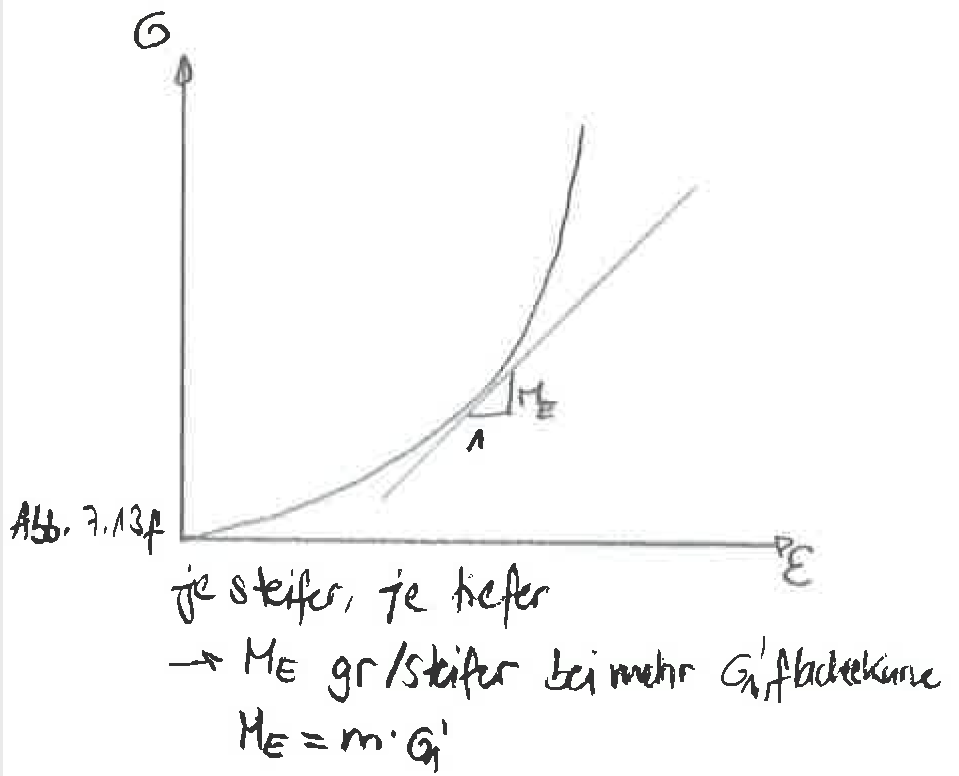
\includegraphics[width=3cm]{images/Kons_1_Sp-Dehnungs-Diagramm}
%		\caption{}
%		\label{fig:kons1sp-dehnungs-diagramm}
%	\end{figure}
%\end{minipage}

\begin{minipage}{\linewidth}
	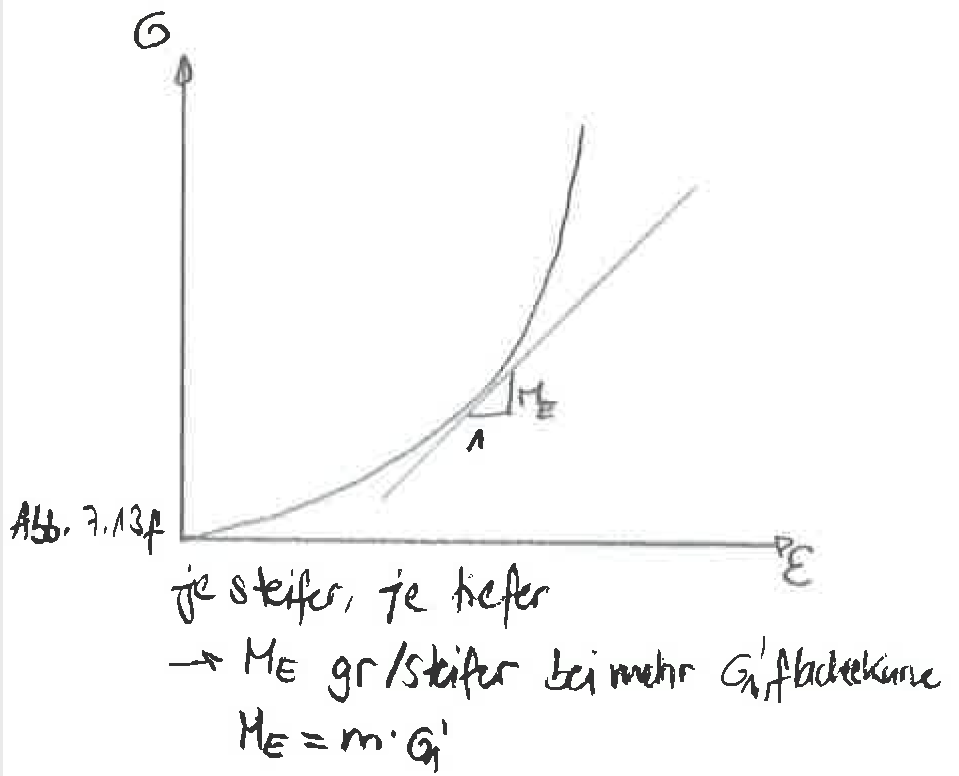
\includegraphics[width=0.4\linewidth]{images/Kons1SpDehnungsDiagramm} \qquad
	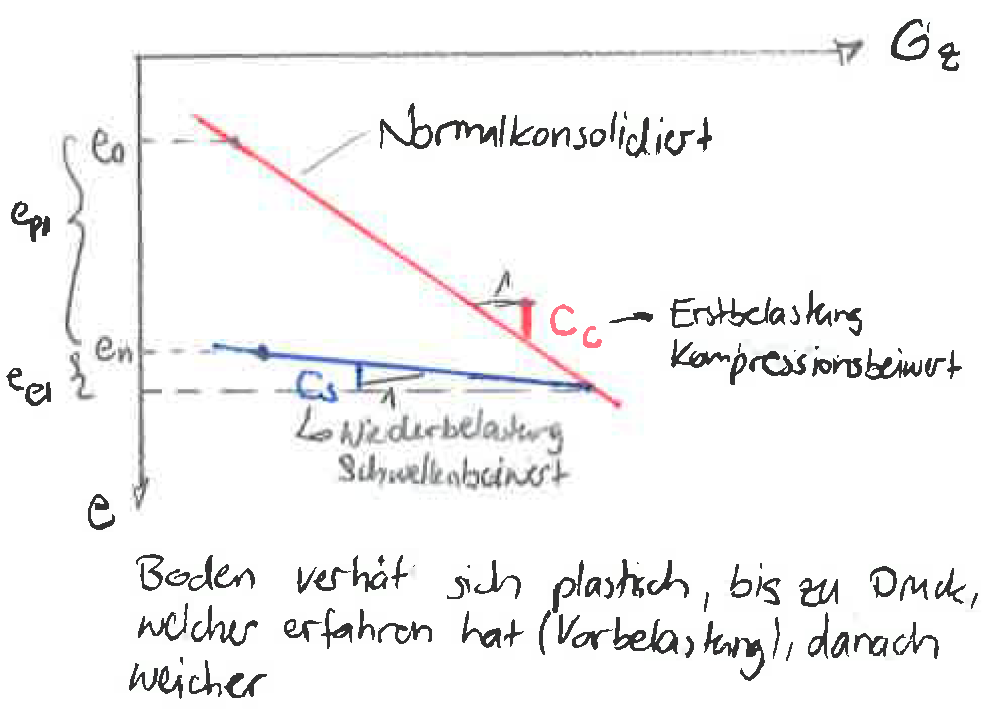
\includegraphics[width=0.4\linewidth]{images/Kons2SPPorenDiagrammCcCs.PNG}
\end{minipage}

\begin{minipage}[t]{0.25\linewidth}	
	\subsection{Umrechnungen}
	\begin{tabular}{|l|l|}
	\hline
	kPa 				& $\frac{kN}{m^2}$ \\ \hline
	Pa					& $\frac{N}{m^2}$  \\ \hline
	kg					& 10 N				\\ \hline
	$\frac{kN}{m^3}$	& $10 \cdot \frac{g}{cm^3}$ \\ \hline
	$\frac{kN}{m^2}$	& $\frac{N}{mm}$	\\ \hline
	$\gamma_w=\frac{kN}{m^3}\cdot 10^{-6}$ & $\frac{kN}{cm^3}$ \\ \hline
	$M_E=\frac{kN}{m^2}\cdot 10^{-4}$ & $\frac{kN}{cm^2}$	\\ \hline
	\end{tabular}
\end{minipage}
\begin{minipage}[t]{0.5\linewidth}
	\subsection{Materialverhalten mit Oedometer}

	\begin{tabular}{l|l|l}
				& Formeln 									& Einheiten \\ \hline \hline
	
		Dehnung &$\varepsilon = \frac{\Delta h}{h_0}$& \\ \hline
	
		Porenziffer&$\e_0=\frac{\gamma_s}{\gamma_d} -1$		& \\
				&$e=e_0-\varepsilon \cdot \left(1+ e_0\right)$	&\\
				&$\rightarrow\frac{\Delta h}{h}=\frac{e_0 - e}{1+e_0}$&\\	
				&$\rightarrow\Delta h=\frac{\Delta \sigma \cdot h_0}{M_E}$&m \\ \hline
	
		$M_E$-Modul&$M_E=\frac{\Delta \sigma}{\Delta \varepsilon}=\frac{1+e_0}{C_c \cdot 0.434}\cdot\sigma_m$&$\frac{kN}{m^2}$ \\	
				&$\rightarrow \gamma_d=\frac{\gamma}{1+w}$	&$\frac{kN}{m^3}$ \\
				&$\rightarrow n=\frac{\gamma-\gamma_d}{S_r\cdot\gamma_w}$&  $_{Porositaet}$ \\
				&$\rightarrow e_0=\frac{n}{1-n}$			& \\
				&$\rightarrow \gamma=\frac{G}{V}\cdot g$	& $\frac{kN}{m^3}$ \\
				&$\rightarrow \gamma_s=$16-17				& $\frac{kN}{m^3}$ \\ \hline

		$\rightarrow$ Oedometer&$\sigma=M_E \cdot \varepsilon$ &$\frac{kN}{m^2}$ \\
				&$\rightarrow M_E\neq E, \hspace{0.25cm}\text{da} \hspace{.25cm} \varepsilon_2=\epsilon_3=0$& \\
				&$\sigma_m=\frac{2\cdot\sigma_0+\Delta \sigma}{2}$&$\frac{kN}{m^2}$ \\ \hline

		Konsolidationskoeffizient&$C_v=\frac{M_E\cdot k}{\gamma_w}=\frac{T_v\cdot d^2}{t}$&$\frac{m^2}{s}$ \\ \hline

		Durchlässigkeitswert&$k=\frac{C_v\cdot\gamma_w}{M_E}$& $\frac{m}{s}$ \\ \hline
		Zeitfaktor&$T_V=\frac{t\cdot C_V}{d^2}=\frac{t\cdot M_E\cdot k}{\gamma_w\cdot d^2}$& \\ \hline
	
		Kompressionsbeiwert&$C_c=\frac{e_2-e_3}{log\frac{\sigma_3}{\sigma_2}}=\frac{2,3\cdot(1+e_0)}{E}\cdot\sigma_{ref}$ &$\sigma_{ref}$ häufig 100kPa\\
				&$C_c=0.009\cdot(w_L-10\%)$					&  \\ 
	
		Schwellenbeiwert& C$_s$								& \\ \hline
		Überkonsolidationsverhältnis		&$OCR=\frac{\sigma_0}{\sigma_{max}}=\frac{Jetzige}{Max.}$ & \\ \hline
		M$_{Platte}$ & $\frac{m\cdot (m^2-m-2)}{(m^2-1)\cdot (m-1)}$ & \\
		$\rightarrow$ kleiner als M$_{E,Oed}$		& $m=\frac{1}{\nu}$							& $\nu=$Querdehnungszahl \\ \hline		
	\end{tabular}
%	\textbf{Dehnungs-Spannungs-Diagramm; Spannungs-Porenziffer-Diagramm (mit Cc \& Cs); Merkmale ME, Verhalten} \\
	\end{minipage}

\clearpage

	\begin{minipage}{\linewidth}

	\subsection{Eindimensionale Konsolidationstheorie}
	
%\textbf{Zeit-Tiefe-Konoslidationsgrad-Diagramm; Verhalten}\\
		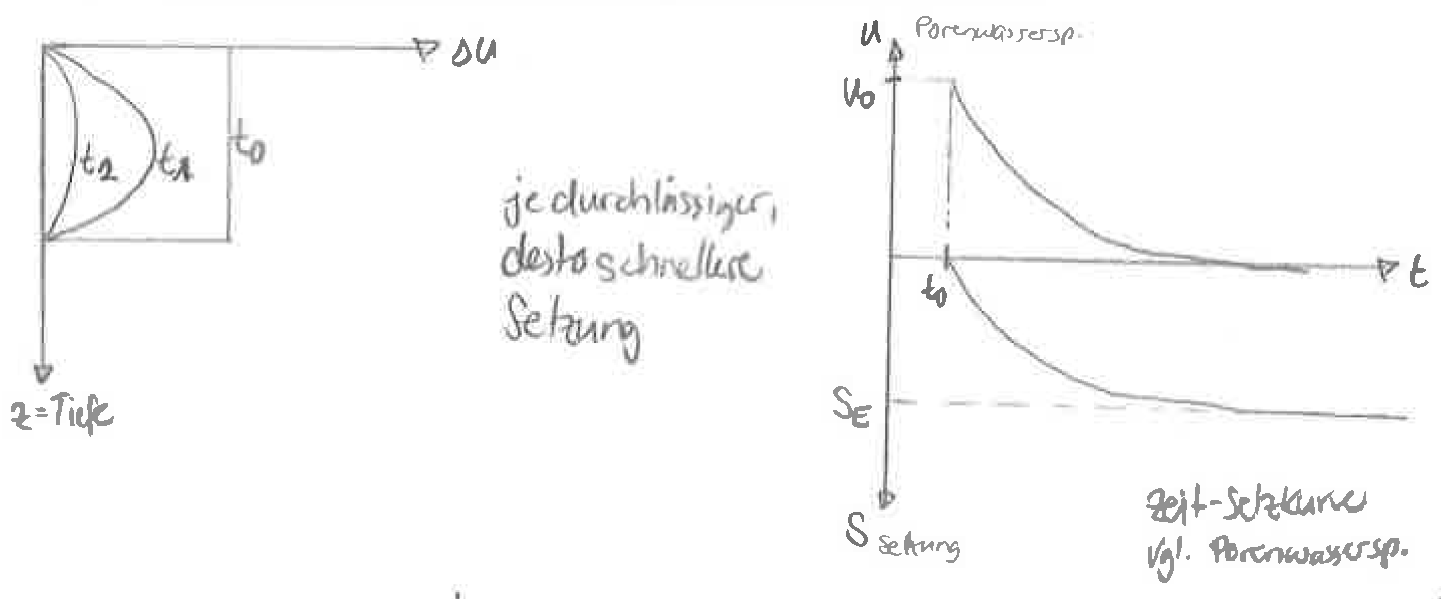
\includegraphics[width=0.7\linewidth]{images/Kons3PorenspTiefZeitSetzungsDiagramm.PNG} \\	
	\begin{tabular}{l|l|l}
				& Formeln											& Einheiten \\ \hline \hline

	Setzungen	& $\Delta s=d^*\cdot \frac{\Delta \sigma}{M_E}$	& m \\
				&													&($d^*=$Weg der Drainage insg. $\rightarrow$ h [m]) \\
				&													&($\Delta\sigma=$Auflast q [kPa][kN/m$^2$]) \\
	Endsetzungen& $\Delta s_{inf}=h\cdot \frac{C_c}{1+e_0}\cdot log\left(\frac{\sigma(0)+\Delta\sigma}{\sigma(0)}\right)$	& m \\ \hline
				
	Konsolidationsgrad & $Um=\frac{\Delta s(t)}{\Delta s_{inf}} = \frac{s_1}{s_E}	$	& \% \\ \hline		

	Terzagi
	(je nach Um)& $T_v=\frac{\pi}{4}\cdot Um^2$ $\rightarrow Um<0.526$& (erwartete Zeit bis Um)\\
				& $T_v=-0.933\cdot log(1-Um)-0.085$ $\rightarrow Um>0.526$& \\
				& $T_v=\frac{c_v \cdot t}{d^2}$						& \\
				& $t=\frac{T_v \cdot d^2}{c_v}$						& s \\
				& $c_v=\frac{k \cdot M_E}{\gamma_w} =\frac{T_v\cdot d^2}{t}$									&$\frac{m^2}{s}$ (Tangente bei Primärsetzungen) \\
				& $\rightarrow$ konst. bei U$_{90}$: $c_v=\frac{d^2 \cdot 0.848}{t_{90}}$& (T$_{v90}=0.848$)\\
				& $c_{\alpha} = \frac{\Delta e}{log \left(\frac{t_2}{t_1}\right)}$ 				& $\frac{m^2}{s}$ (Tangente bei Kriechen)\\ \hline

	Silvaram
	(immer)		& $T_v=\frac{\frac{\pi}{4}\cdot (Um)^2}{\left[1-(Um)^{5.6}\right]^{0.357}}$ & \\	\hline	
	\end{tabular}

\vspace{\baselineskip}
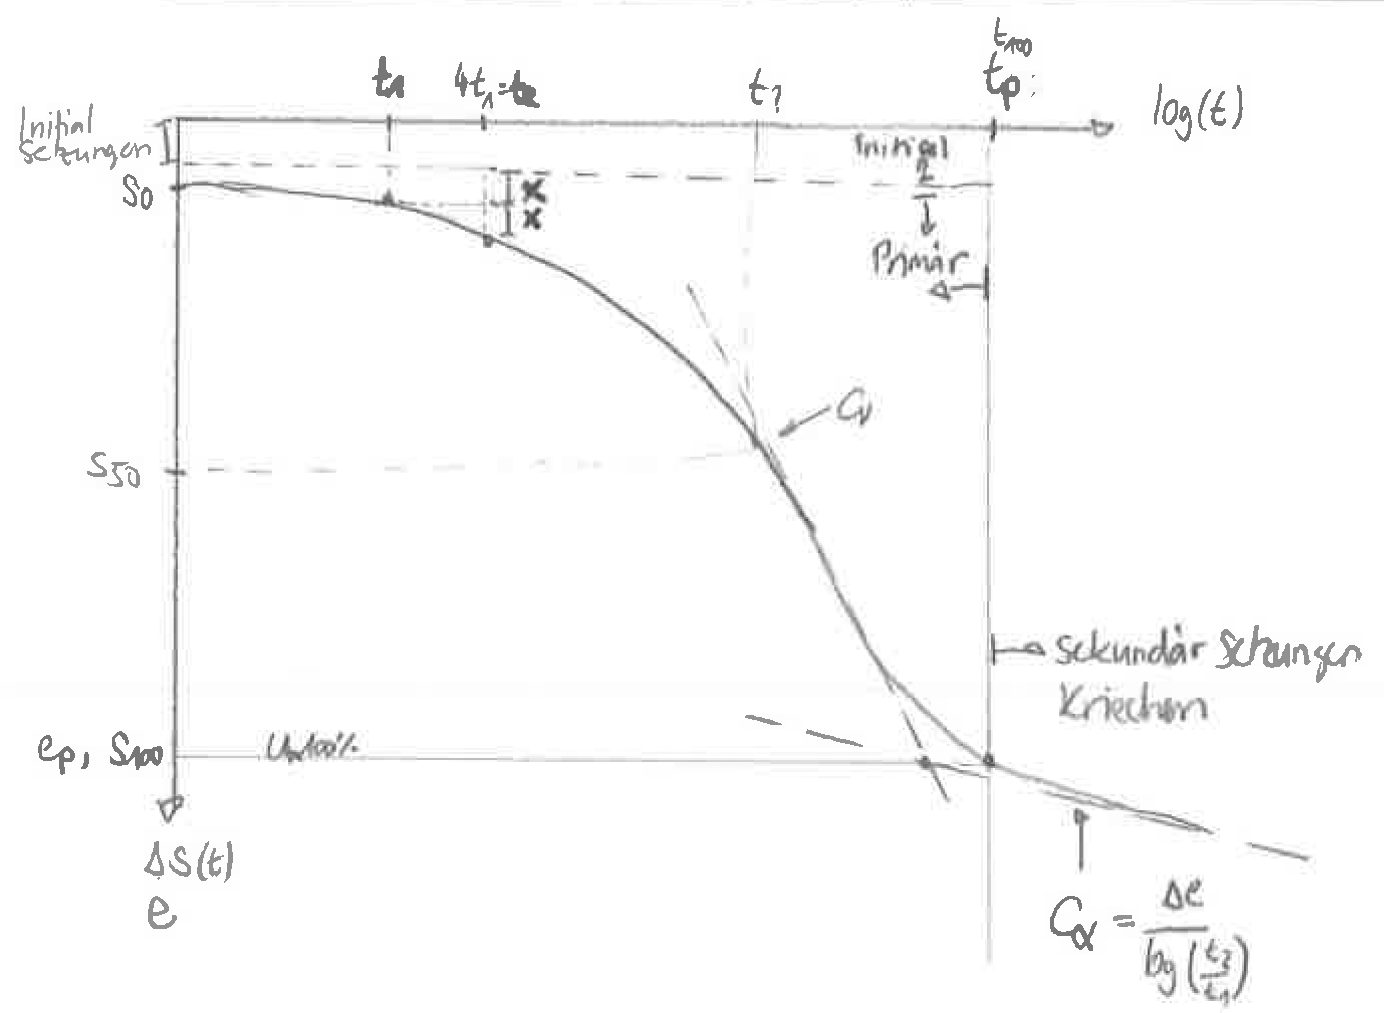
\includegraphics[width=0.6\linewidth]{images/Kons4ZeitSetzungsDiagramm.PNG}
% \textbf{Zeit-Setzungs-Diagramm}
	\end{minipage}